\documentclass[aspectratio=169, 10pt]{beamer}

\usepackage{bm} % bold math
\usepackage{fontspec}
\usepackage{minted}
\usepackage{pgf-pie}
\usepackage{tikz}
\usepackage{graphicx}
\newcommand\sbullet[1][.5]{\mathbin{\vcenter{\hbox{\scalebox{#1}{$\bullet$}}}}}

% Custom commands and environments
\makeatletter
\newcommand\version[1]{\renewcommand\@version{#1}}
\newcommand\@version{}
\def\insertversion{\@version}

\newcommand\course[1]{\renewcommand\@course{#1}}
\newcommand\@course{}
\def\insertcourse{\@course}

\newcommand\coursetitle[1]{\renewcommand\@coursetitle{#1}}
\newcommand\@coursetitle{}
\def\insertcoursetitle{\@coursetitle}

\newcommand\lecturenumber[1]{\renewcommand\@lecturenumber{#1}}
\newcommand\@lecturenumber{}
\def\insertlecturenumber{\@lecturenumber}
\makeatother

\newcommand{\slidetitle}[1]{{\xbseries \large \structure{#1}} \bigskip}
\newcommand{\term}[1]{{\color{blue} #1}}
\newcommand{\leftspace}{\hspace{1em}}
\newcommand{\inlinearrow}{
  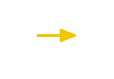
\begin{tikzpicture}[baseline]
    \node [anchor=base] (x) {};
    \draw [rawarrow] (x.mid west) -- ($(x.mid west) + (2em,0)$);
  \end{tikzpicture}
}

\newenvironment{slide}
{\begin{frame}[fragile,environment=slide]\vskip0pt plus 1filll}
{\vskip0pt plus 1filll\end{frame}}

% LaTeX

\setlength{\leftmargini}{1em}

% Common Information

\author{Talia Xu}
\course{COMPSCI 340}
\coursetitle{Operating Systems}
\date{2024 Semester 2}

% fontspec

\defaultfontfeatures{Ligatures=TeX}
% \setmainfont{Domine}
\setsansfont{Inter}[
  FontFace={ul}{n}{Font=*-Thin},
  FontFace={el}{n}{Font=*-ExtraLight},
  FontFace={l}{n}{Font=*-Light},
  FontFace={sb}{n}{Font=*-SemiBold},
  FontFace={eb}{n}{Font=*-ExtraBold},
  FontFace={xb}{n}{Font=*-Black},
]
\setmonofont[Contextuals=AlternateOff, Ligatures=TeXOff]{Iosevka}[
  FontFace={xb}{n}{Font=*-Heavy},
]

%% Font Weights

\DeclareRobustCommand{\ulseries}{\fontseries{ul}\selectfont}
\DeclareTextFontCommand{\textul}{\ulseries}
\DeclareRobustCommand{\elseries}{\fontseries{el}\selectfont}
\DeclareTextFontCommand{\textel}{\elseries}
\DeclareRobustCommand{\lseries}{\fontseries{l}\selectfont}
\DeclareTextFontCommand{\textl}{\lseries}
\DeclareRobustCommand{\sbseries}{\fontseries{sb}\selectfont}
\DeclareTextFontCommand{\textsb}{\sbseries}
\DeclareRobustCommand{\ebseries}{\fontseries{eb}\selectfont}
\DeclareTextFontCommand{\texteb}{\ebseries}
\DeclareRobustCommand{\xbseries}{\fontseries{xb}\selectfont}
\DeclareTextFontCommand{\textxb}{\xbseries}

% tikz

\usetikzlibrary{
  arrows,
  arrows.meta,
  automata,
  backgrounds,
  calc,
  decorations.pathreplacing,
  matrix,
  positioning,
  overlay-beamer-styles,
  shapes,
  shapes.multipart,
  tikzmark,
}

\tikzstyle{rawarrow} = [
  -{Latex[round]},
  line width=1pt,
  yellow,
  shorten >=3pt,
  shorten <=3pt,
  font=\small,
  text=black,
]

\tikzstyle{arrow} = [
  -{Latex[round]},
  line width=1pt,
  yellow,
  shorten >=3pt,
  shorten <=3pt,
  transform canvas={yshift=3pt},
  font=\small,
  text=black,
]

\newcommand{\tikzmarkcoord}[1]{([yshift=3pt]pic cs:#1)}

% minted

\setminted{style=eyolfson, fontsize=\small, escapeinside=||}
\setmintedinline{fontsize=\normalsize}

% hyperref

\hypersetup{colorlinks, urlcolor=blue}

% beamer
\setbeamersize{text margin left=16mm, text margin right=16mm}
\setbeamertemplate{itemize items}[circle]
\setbeamercolor{item}{fg=black}
\setbeamercolor{structure}{fg=darkblue}
\setbeamerfont{frametitle}{series=\bfseries, parent=structure}
\setbeamertemplate{navigation symbols}{}
\setbeamertemplate{headline}{}
\setbeamertemplate{footline}{
  \begin{tikzpicture}[
    remember picture,
    overlay,
    shift={(current page.south west)},
  ]
    \path [fill=gray] (144mm, 0) -- (160mm, 16mm) -- (160mm, 0);
    \node [inner sep=3.5mm, outer sep=0, text=black, anchor=base east,
           align=right, yshift=3.5mm]
          at (current page.south east) {\ttfamily \small \insertframenumber{}};
  \end{tikzpicture}
}
\setbeamertemplate{title page}{
  \begin{tikzpicture}[
    remember picture,
    overlay,
    shift={(current page.south west)},
    background rectangle/.style={fill=darkblue},
    show background rectangle,
  ]
    \node [anchor=center, align=center, text=white, text width=40mm, scale=3.2]
          at (\paperwidth / 2, \paperheight * 2 / 3)
          {\xbseries \inserttitle{}};
    \node [anchor=base west, align=left, inner sep=0, text=white, yshift=2.5mm]
          at (16mm, \paperheight / 3)
          {\insertdate{} \insertcourse{}: \insertcoursetitle{}};
    \node [anchor=base west, align=left, inner sep=0, text=white, yshift=-2.5mm]
          at (16mm, \paperheight / 3)
          {\insertauthor};
    \node [anchor=base east, align=right, inner sep=0, text=white, yshift=2.5mm]
          at (144mm, \paperheight / 3)
          {Lecture \insertlecturenumber{}};
    \node [anchor=base east, align=right, inner sep=0, text=white,
           yshift=-2.5mm]
          at (144mm, \paperheight / 3)
          {\ttfamily \insertversion{}};
    \node [align=center, anchor=south, inner sep=0, text=white, yshift=3.5mm]
          (license) at (\paperwidth / 2, 0)
          {\fontsize{7pt}{7pt}\selectfont This  work is licensed under a
           \href{http://creativecommons.org/licenses/by-sa/4.0/}
                {\color{lightblue} Creative Commons Attribution-ShareAlike 4.0
                 International License}};
  \end{tikzpicture}
}

% xcolor

%% Primary Colour

\definecolor{pantone655}{RGB}{0, 42, 92} % #002a5c
\colorlet{darkblue}{pantone655}

%% Secondary Colours

\definecolor{pantone633}{RGB}{0, 139, 176} % #008bb0
\colorlet{blue}{pantone633}

\definecolor{pantonewarmred}{RGB}{220, 70, 51} % #dc4633
\colorlet{red}{pantonewarmred}

\definecolor{pantone3285}{RGB}{0, 161, 137} % #00a189
\colorlet{cyan}{pantone3285}

\definecolor{pantone7722}{RGB}{13, 83, 77} % #0d534d
\colorlet{darkcyan}{pantone7722}

\definecolor{pantone376}{RGB}{141, 191, 46} % #8dbf2e
\colorlet{green}{pantone376}

\definecolor{pantone2613}{RGB}{109, 36, 122} % #6d247a
\colorlet{violet}{pantone2613}

\definecolor{pantone2985}{RGB}{111, 199, 234} % #6fc7ea
\colorlet{lightblue}{pantone2985}

\definecolor{pantone227}{RGB}{171, 19, 104} % #ab1368
\colorlet{magenta}{pantone227}

\definecolor{pantone7406}{RGB}{241, 197, 0} % #f1c500
\colorlet{yellow}{pantone7406}

%% Neutrals

\definecolor{pantonecoolgray2}{RGB}{208, 209, 201} % #d0d1c9
\colorlet{gray}{pantonecoolgray2}


\lecturenumber{1}
\title{File\\Systems}
\version{1.0.0}

\begin{document}

\begin{frame}[plain, noframenumbering]
    \titlepage
\end{frame}

\begin{slide}

	\slidetitle{Accessing files}
	
	File sharing with socket-based programs
	\bigskip
	
	HTTP, FPT, telnet:
	\begin{itemize}
		\item Explicit access
		\item User-directed connection to access remote resources
	\end{itemize}
	\bigskip
	
	We want more transparency
	\begin{itemize}
		\item Allow user to access remote resources just as local ones
	\end{itemize}
	\bigskip
	
	NAS: Networked Attached Storage

\end{slide}

\begin{slide}

	\slidetitle{Remote File Service Components}
	
	Remote file access network protocol
	\begin{itemize}
		\item Request access to, look up, and access remote files and directories
	\end{itemize}
	\bigskip
	
	Remote file server
	\begin{itemize}
		\item Provides file access interface to clients
	\end{itemize}
	\bigskip
	
	Remote file client (driver)
	\begin{itemize}
		\item Client side interface for file and directory service
		\item File system driver under VFS layer will provide access transparency
		\begin{itemize}
			\item Remote files will be accessed in the same way as local files
		\end{itemize}
	\end{itemize}
	
\end{slide}

\begin{slide}

	\slidetitle{Accessing Remote Files}
	
	For maximum transparency, implement the client module as a file system type under VFS
	\medskip
	
	\includegraphics[width=110mm]{accessing-remote-files.png} 

\end{slide}

\begin{slide}

	\slidetitle{Stateful or Stateless design?}
	
	Stateful: Server maintains client-specific state
	\begin{itemize}
		\item File locking is possible
		\item Better performance in processing requests
	\end{itemize}
	\bigskip
	
	Stateless: Server maintains no information on client accesses
	\begin{itemize}
		\item Each request must identify file and offsets
		\item Server and Client can crash and recover		
		\item Problem if file is deleted on server
	\end{itemize}
	
\end{slide}

\begin{slide}

	\slidetitle{File service model}
	
	Upload/Download model
	\begin{itemize}
		\item Read file: copy file from server to client
		\item Write file: copy file from client to server
		\item Advantage: 
		\begin{itemize}
			\item Simple
		\end{itemize}
		\item Problem: 
		\begin{itemize}
			\item Wasteful: what if client needs small piece?
			\item Problematic: what if client doesn’t have enough space?
			\item Consistency: what if others need to modify the same file?
		\end{itemize}
	\end{itemize}

\end{slide}

\begin{slide}

	\slidetitle{File service model}
	
	Remote access model
	\begin{itemize}
		\item File service provides functional interface
		\begin{itemize}
			\item create, delete, read bytes, write bytes, etc…
		\end{itemize}
		\item Advantage: 
		\begin{itemize}
			\item Client gets only what’s needed
			\item Server can manage coherent view of file system
		\end{itemize}
		\item Problem: 
		\begin{itemize}
			\item Possible server and network congestion
			\item Servers are accessed for duration of file access
			\item Same data may be requested repeatedly
		\end{itemize}
	\end{itemize}

\end{slide}

\begin{slide}
	
	\slidetitle{Semantics of file sharing - Sequential Semantics} 
	
	Read returns result of last write
	
	Easily achieved if
	\begin{itemize}
		\item Only one server
		\item Clients do not cache data
	\end{itemize}
	\bigskip
	
	But
	\begin{itemize}
		\item Performance problems if no cache
		\begin{itemize}
			\item Obsolete data
		\end{itemize}
		\item We can write-through
		\begin{itemize}
			\item Must notify clients holding copies
			\item Requires extra state, generates extra traffic
		\end{itemize}
	\end{itemize}
	
\end{slide}

\begin{slide}

	\slidetitle{Semantics of file sharing - Session Semantics} 

	Relax the rules
	\begin{itemize}
		\item Changes to an open file are initially visible only to the process (or machine) that modified it.
		\item Need to hide or lock file under modification from other clients
		\item Last process to modify the file wins.
	\end{itemize}
	
\end{slide}

\begin{slide}

	\slidetitle{Approaches to caching}
	
	Write-through
	\begin{itemize}
		\item What if another client reads its own (out-of-date) cached copy?
		\item All accesses will require checking with server
		\item Or … server maintains state and sends invalidations
	\end{itemize}
	\bigskip
	
	Delayed writes (write-behind)
	\begin{itemize}
		\item Data can be buffered locally (watch out for consistency – others won’t see updates!)
		\item Remote files updated periodically
		\item One bulk wire is more efficient than lots of little writes
		\item Problem: semantics become ambiguous
	\end{itemize}
	
\end{slide}

\begin{slide}

	\slidetitle{Approaches to caching}
	
	Read-ahead (prefetch)
	\begin{itemize}
		\item Request chunks of data before it is needed.
		\item Minimize wait when it actually is needed.
	\end{itemize}
	\bigskip
	
	Write on close
	\begin{itemize}
		\item Admit that we have session semantics.
	\end{itemize}
	\bigskip
	
	Centralized control
	\begin{itemize}
		\item Keep track of who has what open and cached on each node.
		\item Stateful file system with signaling traffic.
	\end{itemize}
	
\end{slide}

\begin{slide}

	\slidetitle{Case study: NFS}
	
	Network File System
	\bigskip
	
	Sun Microsystems

\end{slide}

\begin{slide}

	\slidetitle{NFS design goals}
	
	Any machine can be a client or server
	\medskip
	
	Must support diskless workstations
	\begin{itemize}
		\item Remote device files refer back to local drivers so we can access our devices
	\end{itemize}
	\medskip
	
	Heterogeneous systems
	\begin{itemize}
		\item Not 100\% for all UNIX system call options
	\end{itemize}
	\medskip
	
	Access transparency: normal file system calls
	\medskip
	
	Recovery from failure
	\medskip
	
	High Performance
	
\end{slide}

\begin{slide}

	\slidetitle{NFS transport protocol}
	
	For the first few versions NFS ran over UDP using Sun Remote Procedure Calls.
	\bigskip
	
	Why was UDP chosen?
	\begin{itemize}
		\item Slightly faster than TCP
		\item No connection to maintain (or lose)
		\item NFS is designed for Ethernet LAN environment - relatively reliable
		\item UDP has error detection (drops bad packets) but no retransmission
			\begin{itemize}
				\item NFS retries lost RPC requests
			\end{itemize}
	\end{itemize}
	
\end{slide}

\begin{slide}

	\slidetitle{NFS: mounting protocol}
	
	Send pathname to server
	\bigskip
	
	Request permission to access contents
	\medskip
	
	\includegraphics[width=70mm]{mounting-protocol-client.png} 
	\medskip
	
	Server returns file handle
	\begin{itemize}
		\item File device \#, inode \#, instance \#
	\end{itemize}
	\medskip
	
	\includegraphics[width=90mm]{mounting-protocol-server.png}
	
\end{slide}

\begin{slide}

	\slidetitle{NFS: directory and file access protocol}
	
	First, perform a lookup RPC
	\begin{itemize}
		\item returns file handle and attributes
	\end{itemize}
	\bigskip
	
	lookup is not like open
	\begin{itemize}
		\item No infromation is stored on server
	\end{itemize}
	
	handle passed as a parameter for other file access functions
	\begin{itemize}
		\item e.g. read(handle, offset, count)
	\end{itemize}

\end{slide}

\begin{slide}

	\slidetitle{NFS Performance}
	
	Usually slower than local
	\bigskip
	
	Improve by caching at client
	\begin{itemize}
		\item Goal: reduce number of remote operations
		\item Cache results of read, readlink, getattr, lookup, readdir
		\item Cache file data at client (buffer cache)
		\item cache file attribute information at client
		\item Cache pathname bindings for faster lookups
	\end{itemize}
	\bigskip
	
	Server side
	\begin{itemize}
		\item Caching is "automatic" via buffer cache
		\item All NFS writes are write-through to disk to avoid unexpected data loss if server dies
	\end{itemize}

\end{slide}

\begin{slide}
	
	\slidetitle{Inconsistencies may arise}
	
	Try to resolve by validation
	\begin{itemize}
		\item Save timestamp of file
		\item When file opened or server contacted for new block
		\begin{itemize}
			\item Compare last modification time
			\item If remote is more recent, invalidate cached data
		\end{itemize}
	\end{itemize}
	\bigskip
	
	Always invalidate data after some time
	\begin{itemize}
		\item After 3 seconds for open files (data blocks)
		\item After 30 seconds for directories
	\end{itemize}
	\bigskip
	
	If data block is modified, it is:
	\begin{itemize}
		\item Marked dirty
		\item Scheduled to be written
		\item Flushed on file close
	\end{itemize}
\end{slide}

\begin{slide}

	\slidetitle{Improving read performance}
	
	Transfer data in large chunks
	\begin{itemize}
		\item 8K bytes default
	\end{itemize} 
	\bigskip
	
	Read-ahead
	\begin{itemize}
		\item Optimize for sequential file access
		\item Send requests to read disk blocks before they are requested by the application
	\end{itemize}
	
\end{slide}

\begin{slide}

	\slidetitle{Problems with NFS}
	
	File consistency
	\medskip
	
	Assumes clocks are synchronized
	\medskip
	
	Open with append cannot be guaranteed to work
	\medskip
	
	Locking cannot work
	\begin{itemize}
		\item Separate lock manager added (but this adds stateful behavior)
	\end{itemize}
	\medskip
	
	No reference counting of open files
	\begin{itemize}
		\item You can delete a file you (or others) have open!
	\end{itemize}

\end{slide}

\end{document}
